%&"main"
% Fakesection 检错
% Fakesubsubsection 宏包
\RequirePackage[l2tabu, orthodox]{nag}
% Fakesubsubsection 编译器
\RequirePackage{ifxetex}
\RequireXeTeX

\documentclass[twoside, openright]{article}
% Fakesection 基础
% Fakesubsection 文字
% Fakesubsubsection 颜色
\usepackage[x11names]{xcolor}
% XXX: conflict with microtype <02-11-19> %
% Fakesubsubsection 长度
\usepackage{printlen}
\uselengthunit{mm}
% Fakesubsubsection 效果
\usepackage{ulem}
% Fakesubsubsection 字体
\usepackage{fontspec}
\setmainfont{Times New Roman}
% XXX: load ctex before siunitx to avoid \ohm ineffective <04-10-19> %
\usepackage[
	UTF8,
	fontset = windows,
	heading = true,
	zihao = -4,
	sub4section,
]{ctex}
\setCJKfamilyfont{zhsong}[
	AutoFakeBold = 2.17,
	AutoFakeSlant = 0.5,
]{SimSun}
\renewcommand*{\songti}{\CJKfamily{zhsong}}
% XXX: load newtxtext before textcomp to avoid option clash <04-10-19> %
\usepackage{newtxtext}
% Fakesubsubsection 字符边框
\usepackage{varwidth}
% Fakesubsection 断行
\usepackage{fvextra}
% Fakesubsection 标点
% XXX: load csquotes after fvextra to avoid warning <04-10-19> %
\usepackage{csquotes}
% Fakesubsubsection Unicode引号样式
\DeclareQuoteStyle{ucstyle}% style name
{\symbol{"201C}}% opening outer mark
{\symbol{"201D}}% closing outer mark
{\symbol{"2018}}% opening inner mark
{\symbol{"2019}}% closing inner mark
% Fakesubsubsection 传统中文样式
\DeclareQuoteStyle{cnzhstyle}% style name
{\symbol{"300E}}% opening outer mark
{\symbol{"300F}}% closing outer mark
{\symbol{"300C}}% opening inner mark
{\symbol{"300D}}% closing inner mark
\setquotestyle{cnzhstyle}
% Fakesubsubsection 书名号样式
\DeclareQuoteStyle{zhtitlestyle}% style name
{\symbol{"300A}}% opening outer mark
{\symbol{"300B}}% closing outer mark
{\symbol{"3008}}% opening inner mark
{\symbol{"3009}}% closing inner mark
% Fakesubsection 样式
% Fakesubsubsection 目录
\usepackage{titletoc}
\titlecontents{section}[0pt]{\filright}{\contentspush{\thecontentslabel}}{}{\titlerule*{.}\contentspage}
% Fakesubsubsection 章节
\ctexset{
	section = {
		name = ,
		number = \arabic{section},
		aftername = \hspace{1\ccwd},
		format = \ifthenelse{\value{section}=0}{\centering}{}\zihao{3}\heiti\bfseries,
		beforeskip = 0.5\ccwd,
		afterskip = 0.5\ccwd,
	},
	subsection = {
		aftername = \hspace{1\ccwd},
		format = \ifthenelse{\value{section}=0}{\centering}{}\zihao{-3}\heiti\bfseries,
		beforeskip = 0.5\ccwd,
		afterskip = 0.5\ccwd,
	},
	subsubsection = {
		format = \zihao{4}\heiti\bfseries,
	}
}
% Fakesubsubsection 图表
\usepackage{caption}
\captionsetup[figure]{labelsep=space}
\captionsetup[table]{labelsep=space}
\captionsetup{font=small}
\DeclareCaptionFont{blue}{\color{LightSteelBlue3}}
\setlength{\abovecaptionskip}{0.5\ccwd}
\setlength{\belowcaptionskip}{0.5\ccwd}
% Fakesubsubsection 子图表
\usepackage{subcaption}
% Fakesubsubsection 公式
\setlength{\abovedisplayskip}{0.5em}
\setlength{\belowdisplayskip}{0.5em}
% Fakesubsubsection 列表
\usepackage{enumitem}
\setlist[enumerate, 1]{
	fullwidth,
	label = (\arabic*),
	font = \textup,
	itemindent=2em
}
\setlist[enumerate, 2]{
	fullwidth,
	label = (\alph*),
	font = \textup,
	itemindent=4em
}
% Fakesubsubsection 代码
% XXX: need -shell-escape & pygmentize <04-10-19> %
\usepackage{minted}
\usepackage{boxie}
% XXX: conflict with fancybox <02-11-19> %
% Fakesubsubsection 问答
\usepackage{exercise}
\usepackage{tasks}
% Fakesubsubsection 改动

% Fakesection 插入
% Fakesubsection 表格
% Fakesubsubsection 三线
\usepackage{booktabs}
% Fakesubsubsection 对角线
\usepackage{diagbox}
% Fakesubsubsection 合并列
\usepackage{multicol}
% Fakesubsubsection 合并行
\usepackage{multirow}
% Fakesubsubsection 分割单元格
\usepackage{makecell}
% Fakesubsubsection 短表
\usepackage{tabu}
% Fakesubsubsection 长表
\usepackage{longtable}
% Fakesubsubsection 彩色表
\usepackage{colortbl}
\usepackage{tcolorbox}
\tcbuselibrary{skins}
\tcbuselibrary{breakable}
\tcbuselibrary{theorems}
\tcbuselibrary{listings}
\tcbuselibrary{xparse}
% XXX: need -shell-escape & pygmentize <04-10-19> %
\tcbuselibrary{minted}
% Fakesubsubsection 导入数据
\usepackage{csvsimple}
% Fakesubsection 图形
% Fakesubsubsection 插图
\usepackage{graphicx}
\graphicspath{{fig/}{etc/}}
% Fakesubsubsection 环绕
\usepackage{wrapfig}
% Fakesubsubsection 图片重叠
\usepackage{overpic}
% Fakesubsubsection 徽标
\usepackage{hologo}
% Fakesubsubsection 条形码
\usepackage{ean13isbn}
% Fakesubsubsection 二维码
\usepackage{qrcode}
% Fakesubsection 符号
% Fakesubsubsection 数学符号
\usepackage{newtxmath}
\usepackage{bm}
% Fakesubsubsection 幻灯片符号
\usepackage{pifont}
% Fakesubsubsection 大数学符号
\usepackage{exscale}
% Fakesubsubsection 数学符号放缩
\usepackage{relsize}
% Fakesubsubsection 公式
\usepackage{cases}
\usepackage{physics}
% Fakesubsubsection 单位
\usepackage{siunitx}
\sisetup{mode=text}
% Fakesubsubsection 计算机
% Fakesubsubsection 音乐
\usepackage{mtxlatex}
\mtxlatex
% Fakesubsection 媒体
\usepackage{media9}
% Fakesubsection 链接
\usepackage[
	colorlinks = true,
	linkcolor = gray,
	citecolor = gray,
	backref = page
]{hyperref}
% Fakesubsection 批注
\usepackage{todonotes}
\usepackage{cooltooltips}
\usepackage{pdfcomment}
% Fakesubsection 文本框
\usepackage{boxedminipage2e}
% Fakesubsection 页眉页脚
\usepackage{fancyhdr}
\fancypagestyle{plain}{
	\pagestyle{fancy}
}

% Fakesection 设计
% Fakesubsection 水印
\usepackage{wallpaper}
% Fakesubsection 主题

% Fakesection 布局
% Fakesubsection 页面
\usepackage{geometry}
% Fakesubsection 缩进
\usepackage{indentfirst}
% Fakesubsection 间距
\usepackage{setspace}
\usepackage[
	restoremathleading=false,
	UseMSWordMultipleLineSpacing,
	MSWordLineSpacingMultiple=1.5
]{zhlineskip}
% Fakesection 引用
% Fakesubsection 脚注
\renewcommand{\thefootnote}{\fnsymbol{footnote}}
\renewcommand{\thempfootnote}{\fnsymbol{mpfootnote}}
% Fakesubsection 引文
\usepackage{morewrites}
\usepackage[square, comma, numbers, super, sort&compress, longnamesfirst, sectionbib, nonamebreak]{natbib}
% Fakesubsection 题注
\usepackage{epigraph}
% Fakesubsection 索引
\usepackage{makeidx}
\makeindex
% Fakesubsection 关联
% XXX: need amsmath <04-10-19> %
%\numberwithin{Exercise}{chapter}
%\numberwithin{Answer}{chapter}

% Fakesection 特殊功能
% Fakesubsection 页数统计
\usepackage{lastpage}
% Fakesubsection 数学表达式
\usepackage{calc}

\begin{document}

% Fakesection 扉页

\newcommand{\Title}{电子电路综合设计}

\begin{titlepage}
	\centering
	\begin{spacing}{1}
		\zihao{4}
		\vspace{0.5\ccwd}

		\vspace{1\ccwd}

		\includegraphics[width=7.41cm]{NJUST.ai}

		\vspace{0.2\ccwd}

		\fontsize{45pt}{45pt}\selectfont\heiti
		\Title

		\zihao{-1}
		\vspace{2\ccwd}
	\end{spacing}

	\begin{spacing}{1.5}
		\zihao{3}
		\begin{tabu} to 12.59cm{@{}X[c, 3.2cm]@{}X[c, 4cm]@{}X[c, 2.22cm]@{}X[c, 3.89cm]@{}}
			\textbf{作  者:} & \underline{\makebox[4cm][c]{\kaishu 吴振宇}} & \textbf{学 号:} & \underline{\makebox[3.89cm][c]{\kaishu 916101630117}} \\
			\textbf{学  院:} & \multicolumn{3}{c}{\underline{\makebox[10.11cm][c]{\kaishu 电子工程与光电技术学院}}} \\
			\textbf{专业(方向):} & \multicolumn{3}{c}{\underline{\makebox[10.11cm][c]{\kaishu 电子信息工程}}} \\
			\textbf{班  级:} & \multicolumn{3}{c}{\underline{\makebox[10.11cm][c]{\kaishu 电信4班}}} \\
			\textbf{题  目:} & \multicolumn{3}{c}{\underline{\makebox[10.11cm][c]{\kaishu 直接数字频率合成器}}} \\
			\textbf{} & \multicolumn{3}{c}{\underline{\makebox[10.11cm][c]{\kaishu}}}
		\end{tabu}
		\vspace{0em}
	\end{spacing}

	\begin{spacing}{1}
		\zihao{3}
		\vspace{3\ccwd}

		\zihao{-3}
		\textbf{指导者:}\underline{\makebox[15.5\ccwd][c]{}}

		\zihao{5}
		\hspace{5em}(姓名)\hspace{11em}(专业技术职务)

		\zihao{-3}
		    \underline{\makebox[15.5\ccwd][c]{}}

		\zihao{5}
		\hspace{5em}(姓名)\hspace{11em}(专业技术职务)

		\zihao{-3}
		\textbf{评阅者:}\underline{\makebox[15.5\ccwd][c]{}}

		\zihao{5}
		\hspace{5em}(姓名)\hspace{11em}(专业技术职务)

		\zihao{3}
		\vspace{2\ccwd}

		\zihao{-2}
		\number\year 年\number\month 月
	\end{spacing}
	\vspace{0em}
\end{titlepage}

% Fakesection 声明

\renewcommand{\abstractname}{\zihao{3}\heiti 声\hspace{2\ccwd}明}
\begin{abstract}
	\zihao{4}

	我声明,本\Title 及其研究工作和所取得的成果是本人在导师的指导下独立完成
	的。研究过程中利用的所有资料均已在参考文献中列出,其他人员或机构对本
	\Title 工作做出的贡献也已在致谢部分说明。

	本\Title 不涉及任何秘密,南京理工大学有权保存其电子和纸质文档,可以借阅
	或网上公布其部分或全部内容,可以向有关部门或机构送交并授权保存、借阅或
	网上公布其部分或全部内容。

	\vspace{2\ccwd}

	\begin{flushright}
		学生签名:\hspace{8em}

		\vspace{1\ccwd}

		年\hspace{3em}月\hspace{3em}日

		\vspace{2\ccwd}

		指导教师签名:\hspace{8em}

		\vspace{1\ccwd}

		年\hspace{3em}月\hspace{3em}日
	\end{flushright}
\end{abstract}

% Fakesection 摘要页眉页脚

\pagestyle{fancy}
\renewcommand{\headrulewidth}{0pt}
\fancyhead[LC, RC]{}
\fancyhead[LE, RO]{}
\fancyhead[RE, LO]{}
\fancyfoot[LC, RC]{}
\fancyfoot[LE, RO]{}
\fancyfoot[RE, LO]{}

% Fakesection 摘要

\newpage

\begin{center}
	\zihao{3}\renewcommand{\CJKglue}{\hskip 2pt}\heiti \Title 中文摘要

	\vspace{0.3em}

	\begin{boxedminipage}[][18cm]{\linewidth}
		\begin{spacing}{1.5}
			\zihao{-4}

			\vspace{1\ccwd}

			本实验利用QuartusII软件设计一个频率及相位均可控制的具有
			正弦和余弦输出的直接数字频率合成器,具有频率控制、相位
			控制、测频、显示多种波形、容量扩展等功能(包含附加功能
			)。实验要求分析整个电路的工作原理,并分别说明了各子模
			块的设计原理,依据各模块之间的逻辑关系,将各电路整合到
			一块,形成一个总体电路。之后再完成调试、仿真、编程下载
			的过程,并对最终结果进行分析,最后总结出在实验过程中出
			现的问题以及提出解决方案。 \cite{王清2010基于FPGA的直接数字频率合成器设计与仿真,杨虹2012简易直接数字频率合成器的设计与仿真,杨小豹2007直接数字频率合成器在}

			\vspace{2\ccwd}

			\noindent\textbf{关键词}\hspace{1\ccwd}直接数字频率合成
			器\hspace{1\ccwd}累加\hspace{1\ccwd}控制\hspace{1\ccwd}
			波形

		\end{spacing}
	\end{boxedminipage}
\end{center}

% Fakesection 英文摘要

\newpage

\begin{center}
	\zihao{3}\renewcommand{\CJKglue}{\hskip 2pt}\heiti \Title 英文摘要

	\vspace{0.3em}

	\begin{boxedminipage}[][18cm]{\linewidth}
		\begin{spacing}{1.5}
			\zihao{3}

			\vspace{1em}

			\begin{tabu} to \linewidth{@{}X[l]@{}X[l, 8]@{}}
				\textbf{Title} & \hspace{2em}\underline{\makebox[15em][c]{\zihao{4}\songti Direct Digital Frequency Synthesizer}} \\
					       & \hspace{2em}\underline{\makebox[15em][c]{\zihao{4}\songti }} \\
			\end{tabu}

			\textbf{Abstract}

			\zihao{-4} In this experiment, QuartusII software is
			used to design a frequency and phase controllable Direct
			digital frequency synthesizer with sine and cosine
			output, with frequency control and phase Control,
			frequency measurement, display of multiple waveforms,
			capacity expansion and other functions (including
			additional functions) The working principle of the whole
			circuit is analyzed and the submodules are explained
			respectively According to the design principle of the
			block and the logical relationship between the modules,
			the circuits are integrated into the One, forming an
			overall circuit. After that, debugging, simulation and
			programming download will be completed. The final
			results are analyzed and summarized in the experimental
			process. Present problems and solutions.

			\vspace{2em}

			\noindent\textbf{Keywords}\hspace{1em} Direct Digital
			Frequency Synthesizer \hspace{1em} Accumulation
			\hspace{1em} Control \hspace{1em} Waveform

		\end{spacing}
	\end{boxedminipage}
\end{center}

% Fakesection 目录页眉页脚

\newpage

\renewcommand{\headrulewidth}{0.4pt}
\fancyhead[LC, RC]{\zihao{-2}\Title}
\fancyhead[LE, RO]{\zihao{5}第\thepage 页}
\fancyhead[RE, LO]{}

% Fakesection 目录

\pagenumbering{roman}

\setcounter{tocdepth}{2}

\renewcommand{\contentsname}{\zihao{3}\heiti 目次}
\tableofcontents
\listoffigures
\listoftables

\newpage
\pagenumbering{arabic}

\section{实验要求}%
\label{sec:实验要求}

设计一个频率及相位均可控制的具有正弦和余弦输出的直接数字频率合成器(Direct
Digital Frequency Synthesizer 简称DDFS或DDS)。

\subsection{基本要求}%
\label{sub:基本要求}

\begin{enumerate}

	\item 利用Quartus II软件和SmartSOPC实验箱实现DDS的设计;

	\item DDS中的波形存储器模块用Altera公司的CycloneIII系列FPGA芯片中的ROM实
		现,ROM结构配置成$ 212\times 10 $类型;

	\item 具体参数要求:频率控制字$ K $取4位;基准频率$ f_c = \SI{1}{\MHz} $
		,由实验板上的系统时钟分频得到;

	\item 系统具有使能功能;

	\item 利用实验箱的D/A转换器件将ROM输出的数字信号转换为模拟信号,能够通过
		示波器观察正弦波形;

	\item 通过开关(实验箱上的$ K_i $)输入DDS的频率和相位控制字,
		并能用示波器观察加以验证。

\end{enumerate}

\subsection{附加要求}%
\label{sub:附加要求}

\begin{enumerate}

	\item 通过按键输入DDS的频率和相位控制字,以扩大频率控制和相位控制的范围;

	\item 能够同时输出正弦余弦两路正交信号;

	\item 在数码管上显示生成的波形频率;

	\item 提高计算精度,考虑到ROM结构及正弦函数的特点。

	\item 设计输出多种波形(三角波、锯齿波、方波等)的多功能波形发生器;

	\item AM调制器的设计。

\end{enumerate}

\section{方案论证}%
\label{sec:方案论证}

\subsection{DDS}%
\label{sub:DDS}

直接数字频率合成器(Direct Digital Frequency Synthesizer)是一种基于全数字技术,
从相位概念出发直接合成所需波形的一种频率合成技术。具有相对带宽大、频率转换时间短
、分辨力高、相位连续性好等优点,很容易实现频率、相位和幅度的数控调制,广泛应用于
通讯领域。

DDS的实际设计中,我们对模拟信号进行采样,获得若干个采样点并存储在存储介质中,输
出时,根据所需要的间隔从存储介质中获取电压量值,并行输出到DAC芯片,芯片输出的电
压即为所还原的信号。其中为了完成对频率和相位的控制,需要在将数字信号转换为模拟信
号的过程中对信号进行额外的处理,经过处理后的信号可以表现出不同的频率和相位甚至不
同的幅度和波形。

\begin{figure}[htbp]
	\centering
	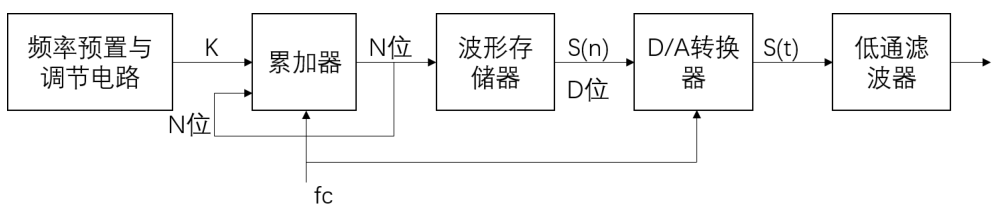
\includegraphics[width=0.8\linewidth]{DDS.png}
	\caption{DDS的组成结构}
	\label{fig:DDS的组成结构}
\end{figure}

由图\ref{fig:DDS的组成结构}可知,DDS的主要由频率预置与调节电路、累加器、波形存储
器、D/A转换器及低通滤波器组成。通过改变频率控制字$ K $可以调节输出信号的频率,$
K $ 越大,输出信号频率越大;相位调节器会对累加器加上一个额外的偏移量,使得输出信
号频率能够得到调节。ROM查找表完成相位到幅度的转换,它接受相位调制器的输出实际上
就是 ROM 的地址值,其输出送入D/A,就得到最终图\ref{fig:DDS的输出流程图}的正弦波
或余弦波。

\begin{figure}[htbp]
	\centering
	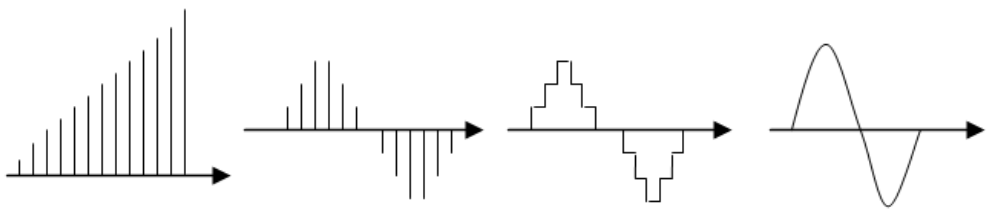
\includegraphics[width=0.8\linewidth]{dia.png}
	\caption{DDS的输出流程图}
	\label{fig:DDS的输出流程图}
\end{figure}

\subsection{理论基础}%
\label{sub:理论基础}

如图\ref{fig:抽样量化的原理}所示,将模拟的正弦函数信号按照一定的周期进行抽样,采
样频率越高,复原出的模拟信号就越精确。由于本次实验采用的是片内ROM的结构配置,实
际中采用了在一个周期内进行1024次采样。

\begin{figure}[htbp]
	\centering
	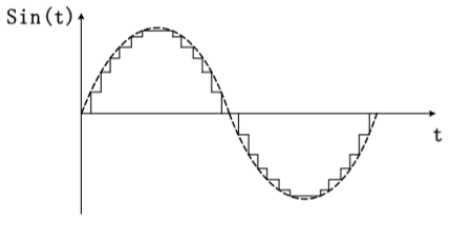
\includegraphics[width=0.8\linewidth]{sample.png}
	\caption{抽样量化的原理}
	\label{fig:抽样量化的原理}
\end{figure}

如图\ref{fig:累加器}所示,直接频率合成器的核心是累加器,将数字信号转换为模拟信号
的过程需要累加,将按照各个步长逐一累加,完成对频率的控制。

\begin{figure}[htbp]
	\centering
	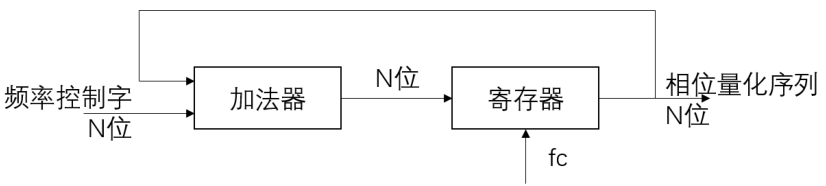
\includegraphics[width=0.8\linewidth]{accumulator.png}
	\caption{累加器}
	\label{fig:累加器}
\end{figure}

如图\ref{fig:低通滤波器}所示,低通滤波器的作用是滤除生成的阶梯形正弦波中的高频成
分,将其变成光滑的正弦波。

\begin{figure}[htbp]
	\centering
	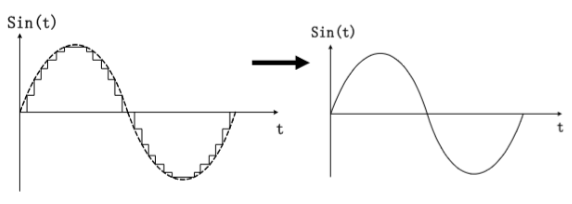
\includegraphics[width = 0.6\linewidth]{lowpass.png}
	\caption{低通滤波器}
	\label{fig:低通滤波器}
\end{figure}

\section{基础功能的各子模块设计原理与实现}%
\label{sec:基础功能的各子模块设计原理与实现}

根据实验要求章节\ref{sec:实验要求},核心电路体框图如图\ref{fig:电路整体框图}。

\begin{figure}[htbp]
	\centering
	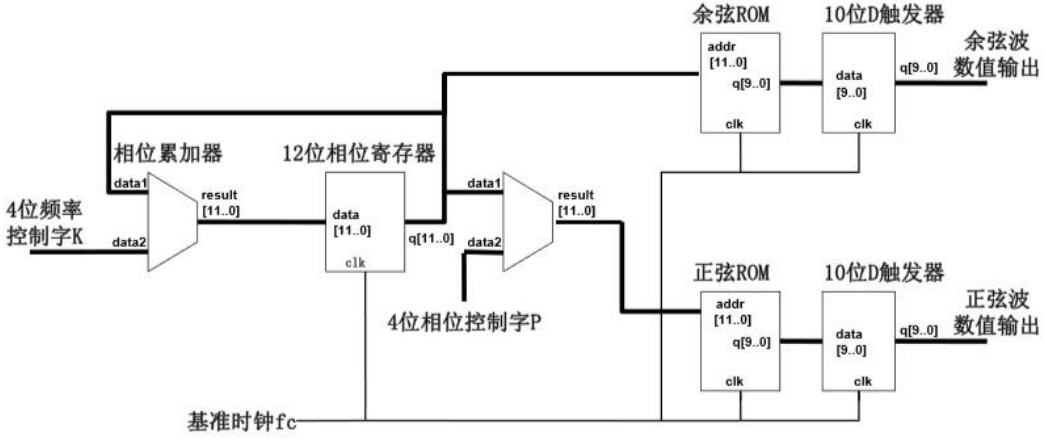
\includegraphics[width=0.6\linewidth]{block.png}
	\caption{核心电路框图}
	\label{fig:核心电路框图}
\end{figure}

电路按功能可细分为以下部分:

\begin{description}

	\item[\nameref{sub:脉冲发生电路}] 通过对主时钟进行分频,产生其它电路所需
		要的时钟频率;

	\item[\nameref{sub:频率调节电路}] 实现输入频率控制字,改变输出信号的频率
		;

	\item[\nameref{sub:相位调节电路}] 实现相位频率控制字,改变输出信号的相位
		;

	\item[\nameref{sub:累加器}] 在时钟的作用下,进行相位累加。;

	\item[\nameref{sub:波形存储电路}] 将经过采样、量化、编码后的波形信号进行存储
		,以便软件能够在需要的时候读取。;

	\item[\nameref{sub:选择波形电路}] 对输出的波形进行选择;

	\item[\nameref{sub:高精度波形电路}] 利用信号的对称性节省 ROM;

	\item[\nameref{sub:消抖电路}] 通过 D 触发器消除颤抖,改善输入信号稳定性
		;

	\item[\nameref{sub:测频电路}] 测量信号频率;

	\item[\nameref{sub:显示译码电路}] 将测频电路的输出数字翻译成数码管的显示
		数字,并采用较高频率的信号使数码管显示译码;

\end{description}

\subsection{脉冲发生电路}%
\label{sub:脉冲发生电路}

脉冲发生电路与多功能数字钟相似,可参照EDA2进行电路的搭建。\footnote{利用HDL 更方
便,但利用EDA2已有的分频电路原理图可以节省开发时间。} 实验板采用的输入脉冲为
\SI{48}{\MHz},所以需要使用分频电路来获得所需频率。

\begin{figure}[htbp]
	\centering
	\begin{subfigure}[htbp]{.45\linewidth}
		\centering
		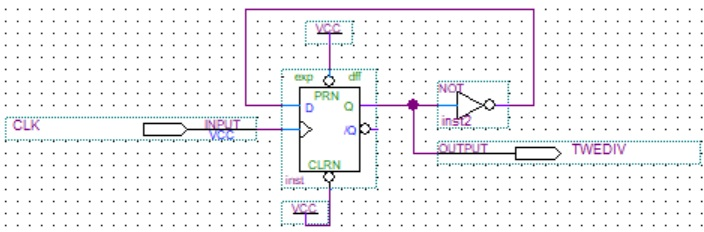
\includegraphics[width=\linewidth]{2.jpg}
		\caption{2分频器}
		\label{fig:2分频器}
	\end{subfigure}
	\quad
	\begin{subfigure}[htbp]{.45\linewidth}
		\centering
		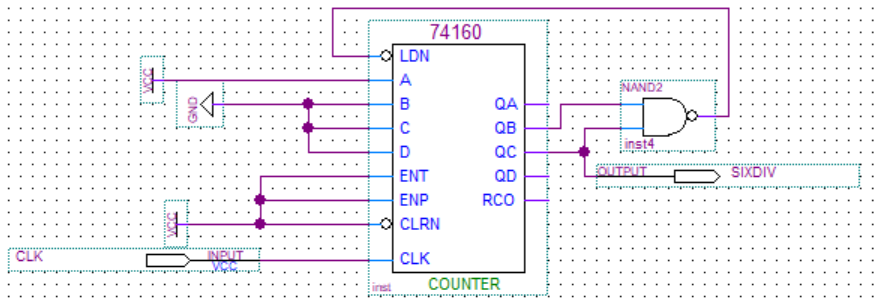
\includegraphics[width = \linewidth]{6.png}
		\caption{6分频器}
		\label{fig:6分频器}
	\end{subfigure}
	\quad
	\begin{subfigure}[htbp]{.45\linewidth}
		\centering
		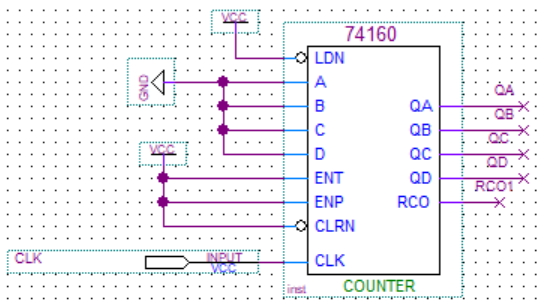
\includegraphics[width = \linewidth]{10.png}
		\caption{10分频器}
		\label{fig:10分频器}
	\end{subfigure}
	\caption{分频器}
	\label{fig:分频器}
\end{figure}

如图\ref{fig:2分频器}所示,二分频器采用一个D触发器和一个非门组成T触发器,其状态
方程为:

\begin{align}
	Q_{n+1} = \overline{Q_n}
\end{align}

每当一个上升沿到来,计数器翻转一次,可对输入信号进行二分频。波形仿真图见图
\ref{fig:2分频器仿真}。

如图\ref{fig:6分频器}所示,6 分频电路由一个 74160 及一个与非门实现,74160 每计数
3 次,置数,使$ Q_\mathrm{C} $端每隔 3 个计数翻转一次。从而实现 6 分频的功能。波
形仿真图见图 \ref{fig:6分频器仿真}。

如图\ref{fig:10分频器}所示,10 分频电路由一个 74160 和一个非门,一个或门,一个与
门实现,74160 每计数 5 次,置数,使 QC 端每隔 5 个计数翻转一次。从而实现 10 分频
的功能。波形仿真图见图 \ref{fig:10分频器仿真}。

\begin{figure}[htbp]
	\centering
	\begin{subfigure}[htbp]{.45\linewidth}
		\centering
		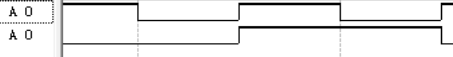
\includegraphics[width = \linewidth]{2-2.png}
		\caption{2分频器仿真}
		\label{fig:2分频器仿真}
	\end{subfigure}
	\quad
	\begin{subfigure}[htbp]{.45\linewidth}
		\centering
		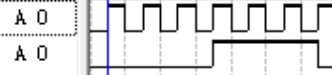
\includegraphics[width = \linewidth]{6-2.png}
		\caption{6分频器仿真}
		\label{fig:6分频器仿真}
	\end{subfigure}
	\quad
	\begin{subfigure}[htbp]{.45\linewidth}
		\centering
		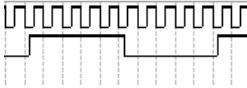
\includegraphics[width = \linewidth]{10-2.png}
		\caption{10分频器仿真}
		\label{fig:10分频器仿真}
	\end{subfigure}
	\caption{分频器仿真}
	\label{fig:分频器仿真}
\end{figure}

\subsection{频率调节电路}%
\label{sub:频率调节电路}

频率调节电路的主要作用是实现输入频率控制字,改变输出信号的频率。频率控制字$ K $
又叫相位增量。DDS的输出频率表达式如式\ref{eq:fout}。

\begin{align}
	f_\mathrm{out} = \dfrac{Kf_\mathrm{c}}{2^N}
		\label{eq:fout}
\end{align}

\begin{wrapfigure}{r}{0.4\linewidth}
	\centering
	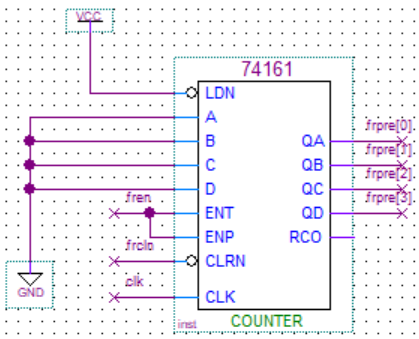
\includegraphics[width=\linewidth]{fr.png}
	\caption{频率调节电路}
	\label{fig:频率调节电路}
\end{wrapfigure}

当$ K = 1 $时,输出最低频率为$ \dfrac{f_\mathrm{c}}{2^N} $;而 DDS的最高输出频率
由Nyquist采样定理决定,$ f_\mathrm{out} = \dfrac{f_\mathrm{c}}{2} $,当$ K =
2^{N-1} $ 时;此时$ K $为最大值。频率控制字设计的是从0000到 1111的四位二进制数,
但是为了与相位累加器的12位二进制相匹配,只需将数值与累加器低四位相加即可,即$ K
$ 的范围是从0000 0000 0000到0000 0000 1111。若直接用开关输入则需要4个开关,而
SmartSOPC实验箱提供的只有 8个开关,为了节省开关,如图 \ref{fig:频率调节电路 }所
示,利用一个模16计数器来产生频率控制字。计数频率采用\SI{1}{\Hz},1秒钟计一次数,
通过开关来控制使达到需要的频率控制字,控制字的数值使用数码管显示出来。

\subsection{相位调节电路}%
\label{sub:相位调节电路}

相位控制模块与频率控制电路较为相似,将计数器的 4 位二进制与累加器的高四位相加,
其低 8 位补零,便得到了相位控制电路。同样为了节省开关其中清零与保持端分别由开关
控制,以便得到所需相位。如图\ref{fig:相位调节电路}所示,相位控制模块与频率控制电
路较为相似,将计数器的4位二进制与累加器的高四位相加,其低8位补零,便得到了相位控
制电路。同样为了节省开关其中清零与保持端分别由开关控制,以便得到所需相位。

\begin{figure}[htbp]
	\centering
	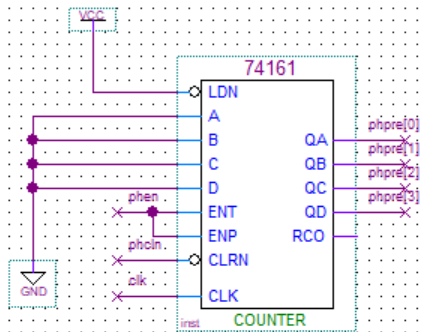
\includegraphics[width = 0.4\linewidth]{ph.png}
	\caption{相位调节电路}
	\label{fig:相位调节电路}
\end{figure}

\subsection{累加器}%
\label{sub:累加器}

相位累加器由加法器和寄存器组成。在时钟的作用下,进行相位累加。当相位累加器累加满
量时就会产生一次溢出,完成一个周期性的动作。输入频率控制字,每接收到一个时钟上升
沿,加法器就会将数据送入寄存器,从而对存储器ROM进行寻址。

使用硬件描述语言能非常简单的完成12位加法器和12位寄存器的设计。

\langCVfile[verilog][lst:verilog/adder12.v][verilog]{verilog/adder12.v}{lst/verilog/adder12.v}

\langCVfile[verilog][lst:verilog/reg12.v][verilog]{verilog/reg12.v}{lst/verilog/reg12.v}

\subsection{波形存储电路}%
\label{sub:波形存储电路}

波形存储电路是一个只读存储器,其作用是将经过采样、量化、编码后的波形信号进行存储
,以便软件能够在需要的时候读取。新建的mif文件输出为10bit ,能够与DAC的输入信号吻
合,使DAC能够输出最低量程到最高量程的电压信号。ROM存储器内存放的值为0到1023 ,共
1024个值。

波形存储器可以存储正弦波,三角波,锯齿波和方波等的数字量。先利用Matlab 生成对应
波形的数据,再通过文件读取的函数将数据写到mif文件中。

\begin{align}
	y = 512\left \lfloor \sin\dfrac{2\pi n}{4096} \right \rfloor + 512
\end{align}

\langCVfile[Matlab][lst:matlab/function/sinwave.m][Matlab]{function/sinwave.m}{lst/matlab/function/sinwave.m}

\begin{align}
	y = 512\left \lfloor \cos\dfrac{2\pi n}{4096} \right \rfloor + 512
\end{align}

\langCVfile[Matlab][lst:matlab/function/coswave.m][Matlab]{function/coswave.m}{lst/matlab/function/coswave.m}

\begin{numcases}{y = }
	1023 & $ 0 \leqslant n \leqslant 2047 $\\
	0 & $ 2047 < n \leqslant 4095 $
\end{numcases}

\langCVfile[Matlab][lst:matlab/function/squarewave.m][Matlab]{function/squarewave.m}{lst/matlab/function/squarewave.m}

\begin{numcases}{y = }
	\left \lfloor \dfrac{n}{2} + 512 \right \rfloor & $ 0 \leqslant n \leqslant 1023 $\\
	\left \lfloor 1024 - \dfrac{n}{2} + 512 \right \rfloor & $ 1023 < n \leqslant 3071 $\\
	\left \lfloor \dfrac{n}{2} + 512 - 2048 \right \rfloor & $ 3071 < n \leqslant 4095 $
\end{numcases}

\langCVfile[Matlab][lst:matlab/function/trianglewave.m][Matlab]{function/trianglewave.m}{lst/matlab/function/trianglewave.m}

\begin{align}
	y = \left \lfloor \dfrac{n}{4} \right \rfloor
\end{align}

\langCVfile[Matlab][lst:matlab/function/sawtoothwave.m][Matlab]{function/sawtoothwave.m}{lst/matlab/function/sawtoothwave.m}

\langCVfile[Matlab][lst:matlab/main.m][Matlab]{main.m}{lst/matlab/main.m}

由于mif文件中的数字由二进制转换而得,故其不能存放浮点数,将采样值使用round函数取
整之后,存储在波形存储器中才可以。

将mif文件写入波形存储器中。在ROM设置中输入地址线 A为12,输出数据D 为10位,之后选
择已经保存好的mif文件,则可以生成波形存储电路如图\ref{fig:波形存储电路}所示:

\begin{figure}[htbp]
	\centering
	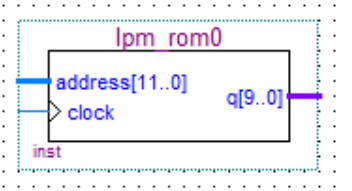
\includegraphics[width=0.4\linewidth]{lpm-rom.png}
	\caption{波形存储电路}
	\label{fig:波形存储电路}
\end{figure}

\subsection{选择波形电路}%
\label{sub:选择波形电路}

为了实现利用实验箱上的 D/A 转换器件将 ROM 输出的数字信号转换为模拟信号,能够通过
示波器观察到正、余弦两路波形;需要对输出的波形进行选择。

\langCVfile[verilog][lst:verilog/xuanbo.v][verilog]{verilog/xuanbo.v}{lst/verilog/xuanbo.v}

\begin{figure}[htbp]
	\centering
	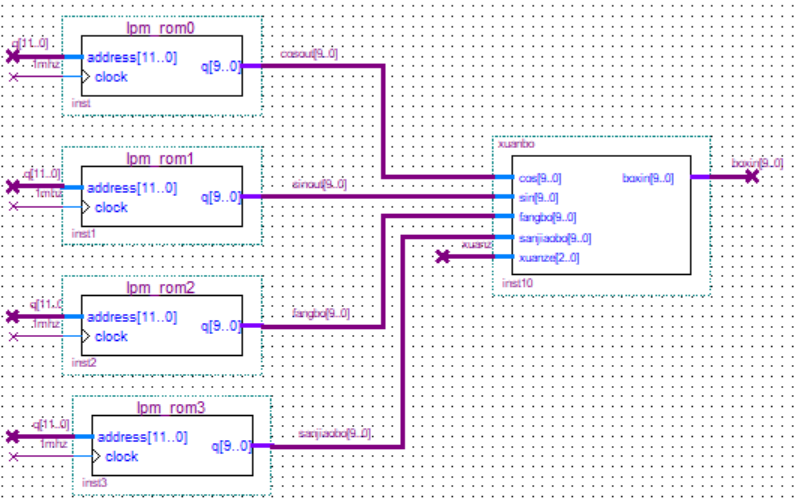
\includegraphics[width = 0.7\linewidth]{select.png}
	\caption{选择波形电路}
	\label{fig:选择波形电路}
\end{figure}

\subsection{高精度波形电路}%
\label{sub:高精度波形电路}

如图\ref{fig:高精度波形电路}所示,以正弦波函数为例,根据正弦波函数的特点,在一个
周期内,每2个$ \dfrac{1}{4} $ 周期之间都存在关系,均可以用$ (0, \dfrac{\pi }{4})
$ 的函数值来表示,根据正弦波的前 $ \dfrac{1}{4} $周期建立mif文件,并生成lpm-rom
,从而实现节省 ROM的高精度波形电路。

\begin{figure}[htbp]
	\centering
	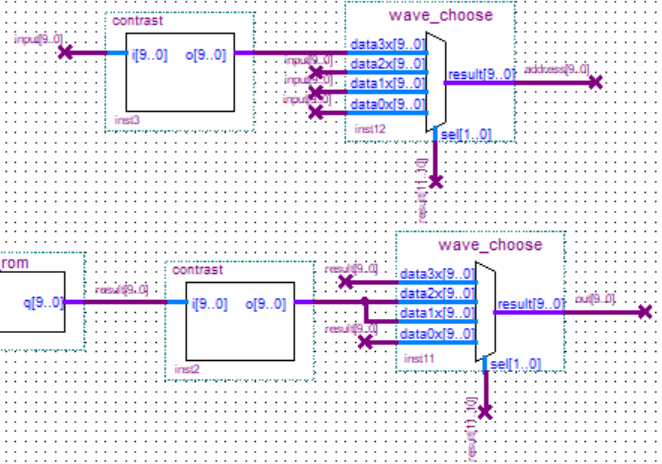
\includegraphics[width = 0.7\linewidth]{precision.png}
	\caption{高精度波形电路}
	\label{fig:高精度波形电路}
\end{figure}

\subsection{消抖电路}%
\label{sub:消抖电路}

如图\ref{fig:消抖电路}所示,将开关连接到 D 触发器的输入端后,颤抖明显被消除,输
入信号稳定性得到改善。

\begin{figure}[htbp]
	\centering
	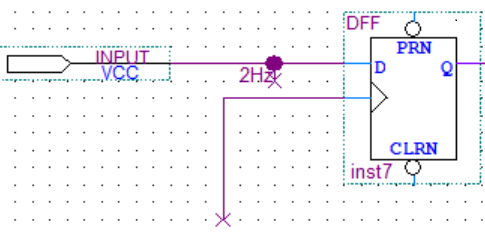
\includegraphics[width = 0.6\linewidth]{tremble.png}
	\caption{消抖电路}
	\label{fig:消抖电路}
\end{figure}

\subsection{测频电路}%
\label{sub:测频电路}

如图\ref{fig:测频电路}所示,测频即测量\SI{1}{\s}内信号经过多少周期,即测试波形存
储器输出最高位的下降沿次数。采用在将累加器输出最高位作为计数器的计数,动态锁存、
显示和复位。

\begin{figure}[htbp]
	\centering
	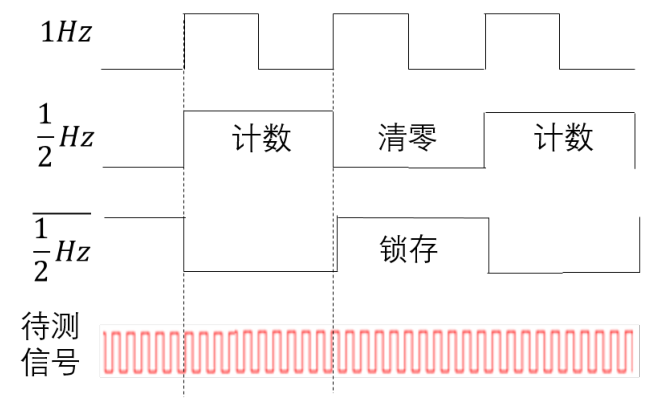
\includegraphics[width = 0.8\linewidth]{measure.png}
	\caption{测频电路}
	\label{fig:测频电路}
\end{figure}

使用单位脉冲信号和计数器即可对频率进行测量。由于测量信号的时间是\SI{1}{\s},故采
用 \SI{0.5}{\Hz} 信号进行状态计数,其高电平正好是\SI{1}{\s},在高电平期间计数,
得到待测信号频率。累加器在每个周期都会溢出一次,将该信号接入测频电路,测量其频率
便可得当前输出信号的频率。

\langCVfile[verilog][lst:verilog/measure.v][verilog]{verilog/measure.v}{lst/verilog/measure.v}

\subsection{显示译码电路}%
\label{sub:显示译码电路}

计数器的数值显示在数码管上,需要使用译码器将BCD码译成数码管显示需要的段码,假设
每一个数码管都有属于自己的译码芯片,将会大大增加电路的复杂性,成本也会有所增加。
故采用数码管的显示译码,每次点亮一个数码管,各数码管循环点亮,接入较高频率的信号
使循环速度加快,在人眼看来,每个数码管都是连续点亮的,达到显示译码的效果。每次只
选择四位计数值接入显示译码器,数码管有3-8译码器点亮一位,循环下去就能达到动态显
示的作用。

如图\ref{fig:显示译码电路}所示,显示译码电路由扫描电路和一个 7447 组成,扫描电路
确定此时哪个数码管显示,7447 用于译码。

\langCVfile[verilog][lst:verilog/scan-led.v][verilog]{verilog/scan\_led.v}{lst/verilog/scan-led.v}

\begin{figure}[htbp]
	\centering
	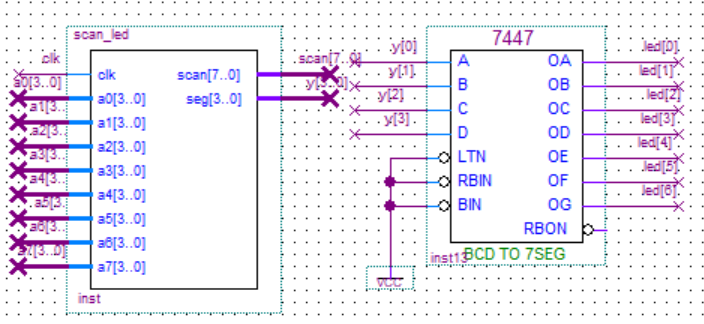
\includegraphics[width = 0.8\linewidth]{display.png}
	\caption{显示译码电路}
	\label{fig:显示译码电路}
\end{figure}

\section{引脚分配}%
\label{sec:引脚分配}

Tcl(Tool Command Language) 是一种脚本语言,QuartusII 支持通过Tcl 自定义功能或自
动执行任务。可以先将引脚设置写在Tcl 中,再导入到项目里。

\langCVfile[Tcl][lst:DDS.qsf][Tcl]{DDS.qsf}{lst/DDS.qsf}

\begin{figure}[htbp]
	\centering
	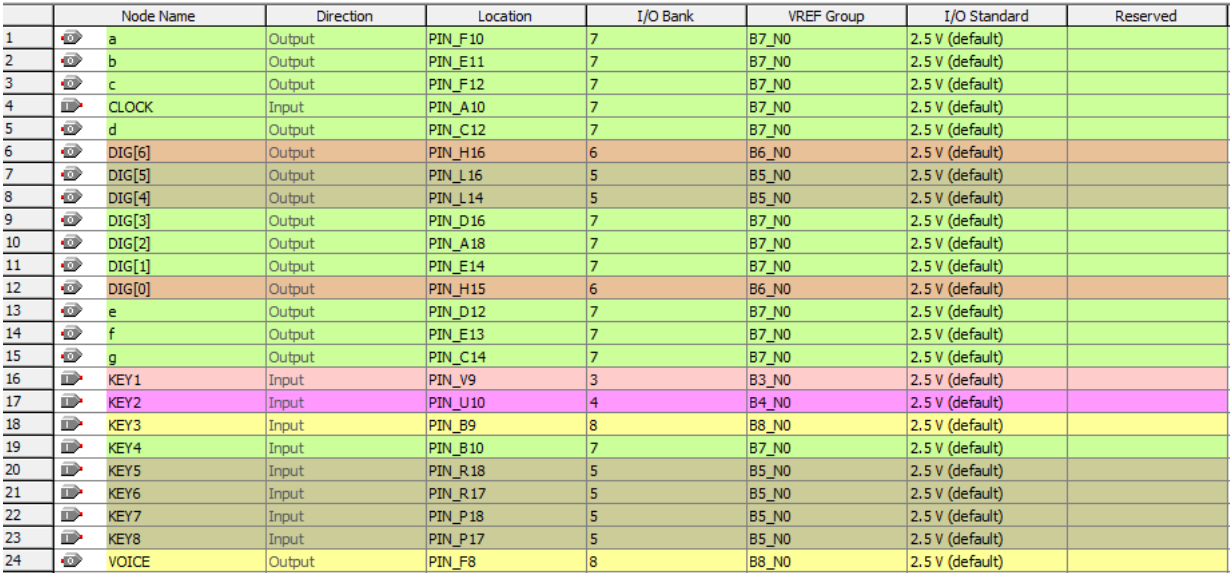
\includegraphics[width = 0.8\linewidth]{pin.png}
	\caption{引脚设置}
	\label{fig:引脚设置}
\end{figure}

将编译好的二进制文件下载进去后可以观察到实验现象如图\ref{fig:实验现象}。

\begin{figure}[htbp]
	\centering
	\begin{subfigure}[htbp]{.45\linewidth}
		\centering
		\includegraphics[width = \linewidth]{sine.jpg}
		\caption{正弦波}
		\label{fig:正弦波}
	\end{subfigure}
	\quad
	\begin{subfigure}[htbp]{.45\linewidth}
		\centering
		\includegraphics[width = \linewidth]{square.jpg}
		\caption{方波}
		\label{fig:方波}
	\end{subfigure}

	\begin{subfigure}[htbp]{.45\linewidth}
		\centering
		\includegraphics[width = \linewidth]{triangle.jpg}
		\caption{三角波}
		\label{fig:三角波}
	\end{subfigure}
	\quad
	\begin{subfigure}[htbp]{.45\linewidth}
		\centering
		\includegraphics[width = \linewidth]{sawtooth.jpg}
		\caption{锯齿波}
		\label{fig:锯齿波}
	\end{subfigure}

	\begin{subfigure}[htbp]{.45\linewidth}
		\centering
		\includegraphics[width = \linewidth]{frequency.jpg}
		\caption{频率调节}
		\label{fig:频率调节}
	\end{subfigure}
	\quad
	\begin{subfigure}[htbp]{.45\linewidth}
		\centering
		\includegraphics[width = \linewidth]{phase.jpg}
		\caption{相位调节}
		\label{fig:相位调节}
	\end{subfigure}
	\caption{实验现象}
	\label{fig:实验现象}
\end{figure}

最终成功地在示波器上观察到了波形,并且通过使用开关控制多路选择器,可以实现不同波
形的切换,获得不同的效果。

\newpage

\section{结论}%
\label{sec:结论}

和上一次EDA实验不同,这一次有了一定的基础,少走了一点弯路。但依旧得到了不少宝贵
的经验教训。

\begin{enumerate}

	\item verilog 作为一门类C 语言语法和C 很像,但本质上依然是一门全新的语言
		,如果照着C 的经验很多地方行不通。譬如,C 语言的自增、自减、取模
		运算符在verilog 中并没有\footnote{在verilog 的超集
		system\_verilog 中引入了这些运算符和更多类C 的语法。};

	\item 在一开始就应该想好一个大致的思路,边想边改非常难,改到最后不如推倒
		重来;

	\item 每次模块内部有改动后,外部必须要更新一次才行。

\end{enumerate}

% Fakesection 参考文献

\setcounter{section}{0}

\addcontentsline{toc}{section}{参考文献}

\bibliographystyle{gbt7714-plain}
\bibliography{bib/main}

\end{document}

